\section{Big Data Analytics - III Lecture}

\subsection{Evolution of Big Data Projects}

\begin{figure}[!h]
  \centering
  \includegraphics[page=38, trim = 3.5cm 1cm 4cm 3.5cm, clip, width=\imagewidth]{images/06 - BIG_DATA.pdf}
\end{figure}

Now, let's discuss the framework for
understanding the evolution of big data projects. Typically, there are
three main types of analytics: descriptive, predictive, and
prescriptive. These analytics require different technologies and
represent different stages of development in handling big data. However,
it's important to note that each stage builds upon the previous ones, so
descriptive analytics are not eliminated in the subsequent steps.

As companies progress in their understanding and utilization of big
data, they go through an evolution from descriptive to prescriptive
analytics. This means that they start with descriptive analytics and
gradually move towards more advanced forms of analysis. By the time a
company completes this evolution, they typically have all types of
analytics integrated into their operations.

\subsection{Descriptive Analytics}

\subsubsection{Traditional Business Intelligence}

Descriptive analytics, also known as traditional business intelligence,
involves taking data and calculating summary indicators based on that
data. This process is similar to what is done in executive information
systems, which we discussed in the BIS1 lecture. In essence, calculating
these indicators is equivalent to running code to provide descriptive
analytics. Therefore, descriptive analytics and traditional business
intelligence can be used interchangeably to refer to this type of
analysis.

\subsubsection{Data Warehousing and Performance}

In our previous discussions, we explored how traditional business
intelligence is enhanced through the creation of a data warehouse. This
allows for the summarization of big data stored in operational
databases, enabling the calculation of descriptive analytics. While
these analytics may not always be instantly available, they can be
efficiently calculated with good performance. In some cases, batch
procedures are used to generate reports, which are then shared either
through a mailing list or a shared document space.

\subsection{Predictive Analytics}

\subsubsection{Decision Making and Predictions}

Companies often progress to the use of predictive analytics to enhance
their decision-making processes. By leveraging their data, they can make
more informed predictions, which serve as the foundation for effective
decision-making. To illustrate the importance of predictions, let's
consider a manufacturing company. Managers in such companies must
determine how many products to produce. However, this decision relies on
an evaluation of future market demand, as the production process often
takes several months. Therefore, accurate predictions of future sales
are crucial. This example demonstrates the connection between
decision-making and the need for predictions.

\subsubsection{Advanced Techniques and Machine Learning}

When companies have accumulated sufficient data and have a reliable
information system in place, they can leverage this data to make
predictions about demand. The demand curve typically fluctuates, and if
the market is growing, there may be an upward trend. To forecast future
demand, companies can analyze the demand curve and trend line to make
predictions. The most common approach is linear modeling, which involves
estimating the trend line and using a linear model to predict growth and
demand.

However, in recent times, companies have started to adopt more advanced
algorithms that go beyond simple trend lines. One example is the use of
machine learning, specifically the random forest algorithm, to predict
sales. Machine learning techniques have been shown to yield better
results by reducing errors. In previous classes, we have explored an
example of using a random forest to predict sales and observed the
improved accuracy that advanced techniques can provide.

\subsection{Prescriptive Analytics}

Once a company has embraced and mastered the use of advanced predictive
analytics, they can begin to trust the analytical predictions based on
data over their own intuition and market knowledge. This is when they
can fully rely on algorithms and receive prescriptions for
decision-making. Moving towards prescriptive analytics involves
automating decisions to some extent.

It is important to note that companies are often hesitant to automate
decisions for various reasons, as we have previously discussed. However,
a prescriptive approach can be applied to less critical decisions,
allowing human decision-making to focus on the most critical ones. These
critical decisions are the ones that change frequently and require
continuous creativity and attention to ensure they are made in the best
possible way.

\subsection{Big Data Challenges}

\subsubsection{Classification of Challenges}

\begin{figure}[!h]
  \centering
  \includegraphics[page=39, trim = 0.3cm 2.5cm 1cm 4cm, clip, width=\imagewidth]{images/06 - BIG_DATA.pdf}
\end{figure}

When it comes to decision-making, there are often choices that go beyond
what individuals can handle due to limited rationality. In these cases,
it becomes necessary to delegate these decisions to machines. However,
this process is not without its challenges. These challenges can be
classified into three main categories: data challenges, process
challenges, and management challenges.

\paragraph{Data Challenges}
Data challenges involve obtaining the necessary data, interpreting it
correctly, and preparing it for the analytics process. This can be a
complex task, as data comes in various formats and from different
sources.

\paragraph{Process Challenges}
Process challenges are related to implementing changes within an
organization to effectively utilize analytics. This involves adapting
existing processes and workflows to incorporate data-driven insights and
recommendations.

\paragraph{Management Challenges}
Lastly, management challenges encompass overseeing the entire process
and ensuring its effectiveness. This includes managing resources,
coordinating teams, and making strategic decisions to maximize the
benefits of analytics.

While all three categories of challenges are important, management
challenges tend to be the most prevalent. This is because effectively
managing the entire process is crucial for achieving successful
outcomes.

By understanding and addressing these challenges, organizations can
navigate the complexities of utilizing big data and make informed
decisions that drive positive change.

\subsubsection{Issues with Big Data Projects}

\begin{figure}[!h]
  \centering
  \includegraphics[page=40, trim = 0cm 3.5cm 1.5cm 4.5cm, clip, width=\imagewidth]{images/06 - BIG_DATA.pdf}
\end{figure}

\paragraph{Technical Skills and Technology Platforms}

One of the main issues in dealing with big data is acquiring the
necessary technical skills to effectively manage the new technologies
involved. While there is a lot of discussion surrounding big data,
companies will struggle to be effective if they lack the technical
expertise required to handle it. In order to perform analytics, the
first step is to have the appropriate technology in place. While it is
possible to run pilot programs or perform some analytics without fully
implementing the technology platform, at some point, it becomes
necessary to adopt the platform. Obtaining the required skills is
crucial in this process.

Cloud computing can be a valuable solution as it provides a ready-to-use
platform for analytics. However, the costs associated with cloud
computing can be a deterrent for many companies. This expense often
leads to reluctance in utilizing cloud computing services.

\paragraph{Data Integration and Preparation}

Data integration and preparation pose significant challenges in the
realm of big data. Often, data is stored in multiple databases that lack
integration and adhere to different standards. This lack of integration
makes the data unfit for analysis. For instance, call center recordings
need to be structured using speech-to-text technology and labeled before
they can be analyzed. Without this preparation, running analytics on the
data becomes impossible.

Furthermore, obtaining useful insights from the data requires a
combination of analytical skills in computer science, business, and
statistics. This presents a management challenge as it is rare to find
all these skills in a single individual. Building a team with diverse
expertise becomes crucial. However, managing such a team can be complex.
It involves finding the right people, fostering a cooperative
environment, and ensuring effective collaboration among team members.
This management challenge is essential for successful data analysis and
utilization.

\paragraph{Management and Organizational Challenges}

Lastly, achieving business involvement is crucial in the process of
transforming an organization through analytics. However, this is not an
easy task. It requires strong motivation from top management, as without
their support, the transformation is unlikely to happen from the bottom
up. Additionally, there will be internal resistance to change, as is
common in any innovation project. This resistance will be even more
challenging to overcome because it involves changing the way managers
work. Unlike automating clerical work, implementing big data and
analytics addresses decision-making processes. Therefore, managers must
recognize the need for support to improve their work, which can be a
difficult mindset to shift.

\subsubsection{Technology Limitations and Scalability}

When it comes to big data, companies face various technical challenges
that require investment in technology. In the past, companies could work
with small data and perform simple analytics using tools like Excel.
Excel was popular because it was user-friendly and flexible, allowing
users to easily calculate indicators and make changes to their
analytics. Managers could independently work with Excel without relying
on the IT department for every request.

However, Excel has its limitations. For instance, it cannot handle
datasets with more than 1 million rows. Opening a CSV file with more
than 1 million rows is not possible in Excel. This limitation poses a
problem when dealing with big data.

\subsubsection{SQL and NoSQL Databases}

One limitation of SQL databases is the number of columns they can
handle. However, this limitation is usually not a major issue when
loading files from an SQL database, as the number of attributes is
typically much lower than the maximum limit of 16,000. The more common
limitation is the number of rows, which is often capped at 1 million.
This means that using Excel to handle such large datasets is not
feasible, as Excel starts to slow down significantly even with just
100,000 rows. The practical maximum for Excel is usually much lower than
1 million rows.

To overcome this limitation, one option is to use a database like MySQL.
However, MySQL caches data in memory and stores it on disk, which means
it can exceed the available RAM on your PC. For example, if you have a
one terabyte hard drive, you can theoretically use the entire space for
data storage. While this may seem like a solution, there is a rule of
thumb to ensure Excel's efficiency: you need to have at least 10\% of
the disk size in memory to achieve optimal performance.

\subsubsection{Oracle Scalability}

\begin{figure}[!h]
  \centering
  \includegraphics[page=45, trim = 1.5cm 1.7cm 1cm 3.5cm, clip, width=\imagewidth]{images/06 - BIG_DATA.pdf}
\end{figure}

If you have one terabyte of data on your disk, MySQL will require 100
gigabytes of RAM to perform well. This means that the limitation is not
the disk, but the memory. When there is not enough memory, MySQL stores
data on disk, which significantly slows down queries. In some cases,
queries may not even converge, causing delays and incomplete results. To
overcome these limitations, you can build a cluster of machines or
consider using cloud computing. However, storing one terabyte in the
cloud and running efficient MySQL queries would require at least 10
servers, resulting in significant costs.

When it comes to scalability, Oracle claims a maximum database size of
eight exabytes, which is a substantial amount. However, in the context
of big data, we haven't reached the exabyte scale in any of the examples
discussed. Oracle offers additional advantages, such as native
integration with NoSQL databases like Hadoop and various analytics
tools, including the open-source R tool. Despite these advantages, it's
important to note that Oracle is an SQL database.

The limitations of SQL databases lie in their approach to handling large
amounts of data. While they offer data dependability and transaction
correctness, their performance can be a disadvantage. To ensure
correctness, data needs to be split into multiple tables, and queries
involving join operations can create scalability issues. Alternative
technologies like IBM Netezza and Teradata offer better performance but
come at a high cost. Another option is the NoSQL paradigm, which allows
for denormalized data storage, reducing the need for join operations.
However, NoSQL databases like Hadoop are optimized for sequential read
and have poor random read performance, making them less suitable for
machine learning algorithms.


\subsubsection{Hadoop Scalability}

\begin{figure}[!h]
  \centering
  \includegraphics[page=48, trim = 1.5cm 7cm 1.5cm 5cm, clip, width=\imagewidth]{images/06 - BIG_DATA.pdf}
\end{figure}

Hadoop, an open-source Apache technology, is not just a database but an
ecosystem of tools. It consists of Hadoop Distributed File System (HDFS)
and MapReduce, which provide a way to query large tables without the
issues faced by SQL databases. Hadoop also includes components like Hive
for running SQL queries, connectors to various analytics environments,
and libraries for machine learning. Commercial distributions like
Cloudera, MapR, and Pivotal offer additional features and simplify
enterprise-level management of Hadoop.

\begin{figure}[!h]
  \centering
  \includegraphics[page=47, trim = 1.5cm 2cm 3cm 5cm, clip, width=\imagewidth]{images/06 - BIG_DATA.pdf}
\end{figure}

However, companies are now questioning the performance and suitability
of Hadoop for all tasks. Its optimization for sequential read and poor
write performance make it challenging to use as a single database
solution. Another challenge is data integration, as companies often have
data scattered across different tools and systems. Data lifecycle
management is also crucial, as data becomes obsolete and needs to be
deleted. This process is more complex in analytical systems, requiring
careful coding to keep data updated and ensure timely deletion.


\subsubsection{Data Science Tools and Automation}

One of the challenges organizations face is acquiring the right skills
for data science. It can be difficult to find skilled data scientists
who can effectively work with computer scientists to extract insights
from data. To address this challenge, there are tools available, such as
KNIME, that enable end-to-end machine learning and automate the data
science cycle. These tools aim to streamline the process by eliminating
the need for coding. Unlike programming languages like R or Python,
which require coding to obtain results, these tools offer a no coding
approach. However, it's important to note that there is still a
significant amount of data preparation required before being able to
upload a clean CSV file into these tools.

\subsubsection{Leadership and Company Culture}

If data preparation is not done correctly, the tools used will not be
effective in providing support or help in correcting data errors. These
tools also have other limitations, such as automatically assigning types
to columns based on the first 10,000 values. However, this can lead to
errors if the type assigned is not accurate for all the data. For
example, a column may be assigned a numeric type, but the 10,001st value
could be a string, causing errors in analysis.

\begin{figure}[!h]
  \centering
  \includegraphics[page=55, trim = 1.5cm 4cm 1cm 4.5cm, clip, width=\imagewidth]{images/06 - BIG_DATA.pdf}
\end{figure}

To overcome these challenges, it is important to have a data scientist
who is not only skilled in statistics but also has computer engineering
skills. Collaboration between data scientists and computer scientists is
necessary for end-to-end automation and efficient data preparation and
maintenance. This highlights the need for a team rather than relying
solely on individual expertise.

Leadership plays a crucial role in addressing these challenges. Clear
goals must be set for the team to ensure effective data preparation and
analysis. Additionally, company culture is an important factor to
consider. A culture that values data-driven decision-making and
encourages collaboration between different teams can greatly contribute
to overcoming these challenges.

Companies often rely on the ``HiPPO decision'', where the highest paid
person's opinion is considered the final say. It's comfortable to have
someone else make decisions for you. However, stepping out of this
comfort zone and being equipped with tools to make informed decisions
can be challenging. Even the highest paid person in the company may
struggle to admit that tools can be helpful. To achieve effective
decision-making, it is crucial to involve the entire business and foster
a data-oriented company culture. This requires significant change
management efforts. Evangelization and taking on big data projects step
by step are essential in this process.
